\begin{figure}[htp]
\begin{center}
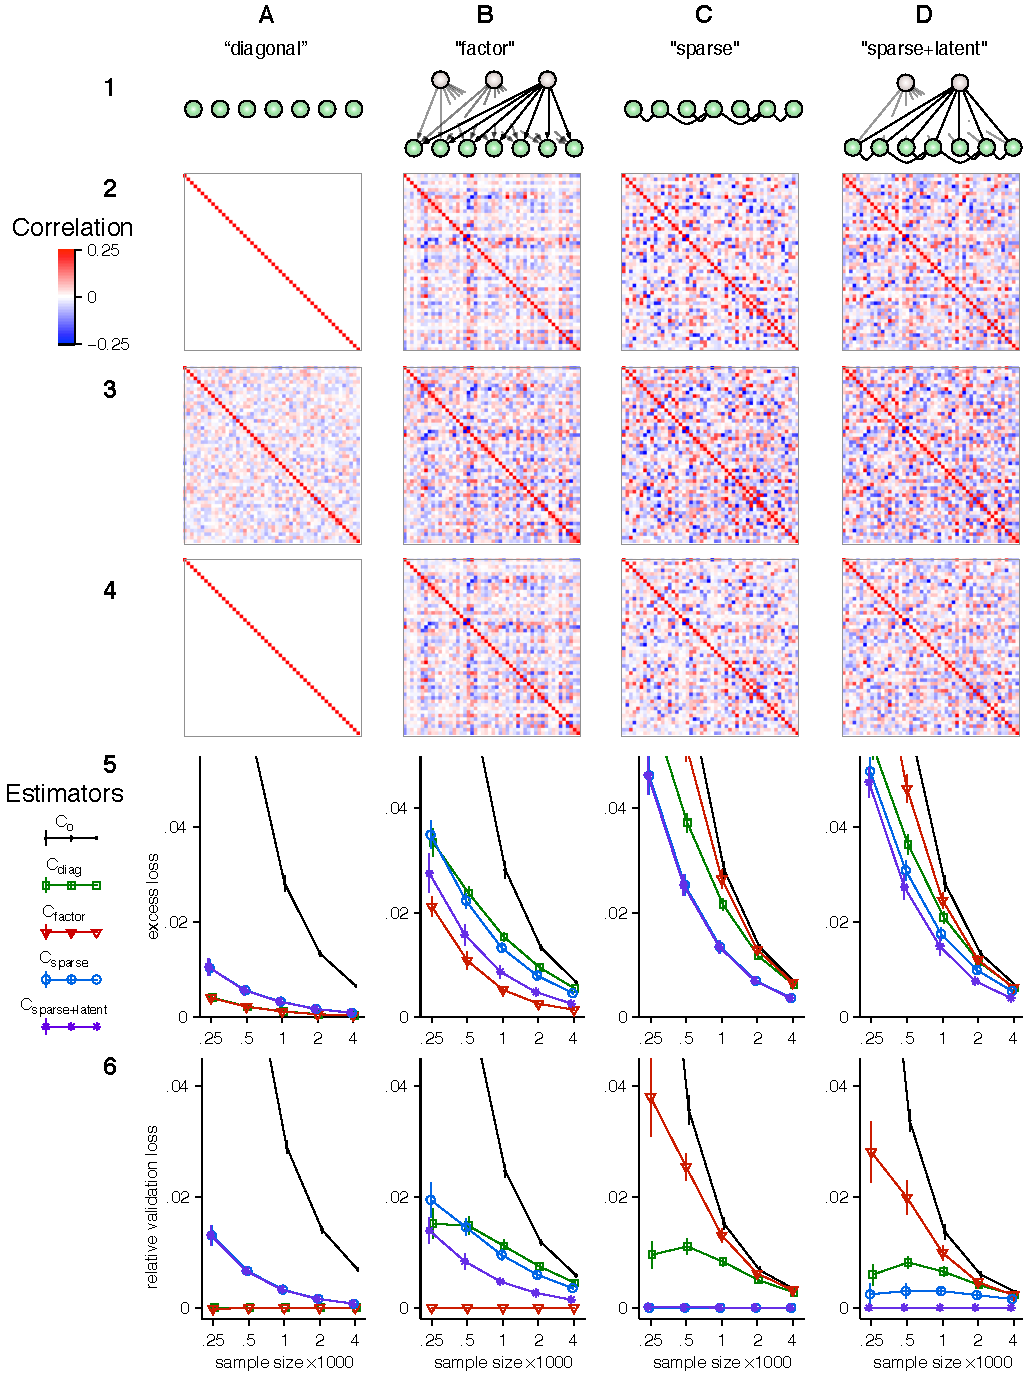
\includegraphics[width=0.5\textwidth]{figures/Figure1.pdf}
\end{center}
\caption{
{\bf Acquistion of neural population activity using two-photon fluorescence imaging of calcium signal.}  {\bf A.} Visual stimuli comprising brief (500 ms) presentatios of full-field drifting gratings separated by blank screens. {\bf B.} Two-photon fast 3D imaging of calcium signals. {\bf C.} The first and last 30 seconds of a 30-minute recording of population calcium signals. The signals are deconvovled and binned at 150 ms. {\bf D.} The sample noise correlation matrix of neuronal calcium signals from {\bf C} after subtracting the average stimulus response. {\bf E.} The hIstogram of off-diagonal coefficients from the correlation matrix in {\bf D}.
}
\label{fig:01}
\end{figure}
